\section{Menu Phase: 2D Renderer}
With the VGA up and running and a robust double buffering system the game finally starts. The player enters the 2D renderer which diplays the menu to setup the 3D game. It is look pretty simple yet features a nice VGA trick.
\par
\begin{figure}[H]
\centering
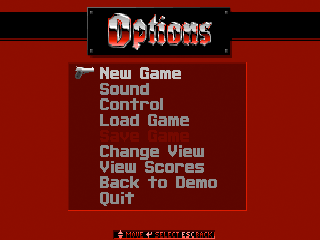
\includegraphics[width=\textwidth]{screenshots/first_menu.png}
\end{figure}
\par


\begin{minipage}{.55\textwidth}
With control over the bank mask, it is possible to write up to four pixels with only one write operation! In the VGA layout to the right, you can see how pixels 0, 1, 2 and 3 are in different banks but at the same address (0x0000). By configuring the bank mask to 8+4+2+1 (15), it is possible to write to all banks simulaneously.\\
\par
Therefore in order to clear the screen to red before drawing the menu, the 2D engine only performs 320x200/4 = 16,000 writes instead of 64,000.\\
\par
\end{minipage}
\begin{minipage}{.4\textwidth}
\begin{figure}[H]
\centering
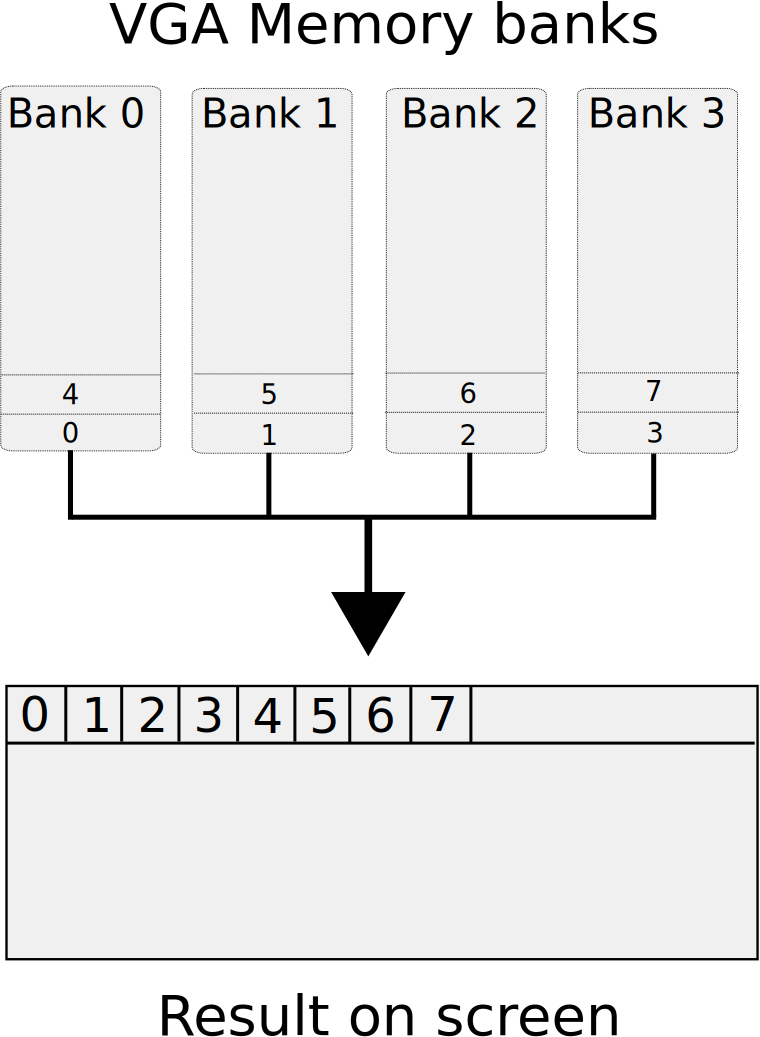
\includegraphics[width=\textwidth]{imgs/drawings/vga_ram_screen_layout.pdf}
\end{figure}
\end{minipage}

\par

\lstinputlisting[language=C]{code/vga_clear/optimal.c}

There is a limitation to this trick of course: Only bytes at the same address in a bank can be populated. Pixel alignment with banks has to be carfully considered. In a layout as follow\\
\par
\begin{figure}[H]
\centering
 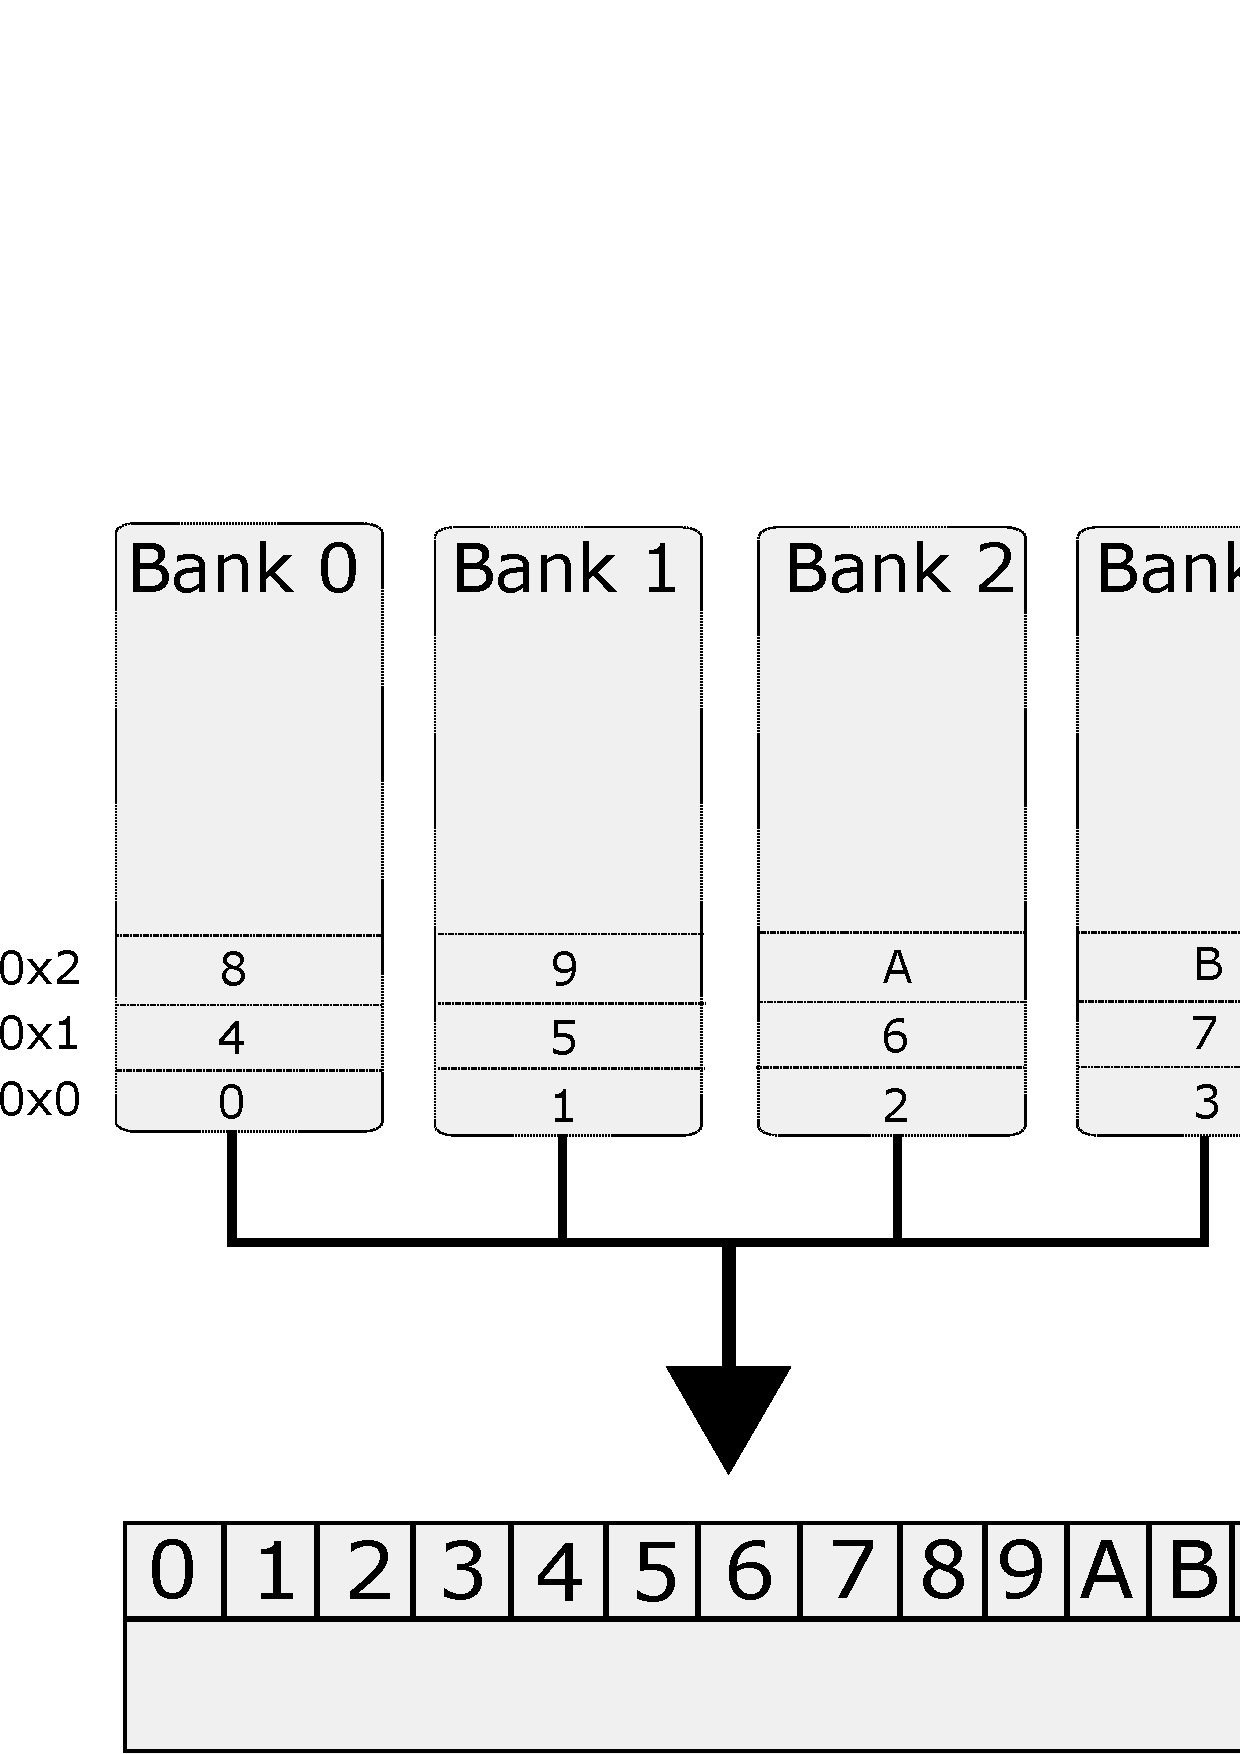
\includegraphics[width=.7\textwidth]{imgs/drawings/scalePost_explanation1.pdf}
 \end{figure}
Pixels 0, 1, 2, 3 can be written in one write.\\
Pixels 3 and 4 need two write operations.\\
Pixels 3, 4, 5, 6, 7, 8 would need three.\\


\par
The rest of the 2D renderer is pretty straigh forward. It uses extensively the US Manager to render font and the Cache manager to retrieve the assets from HDD. Assets are called "pic" as opposed to "sprites" in 3D renderer. Pics are all Huffman-compressed (VGADICT, VGAHEAD, VGAGRAPH).
\par
\note{Where do i mention the bug with assets wrong id in meny (gun replaced by hero.)?}